% This is sigproc-sp.tex -FILE FOR V2.6SP OF ACM_PROC_ARTICLE-SP.CLS
% OCTOBER 2002
%
% For tracking purposes - this is V2.6SP - OCTOBER 2002

\documentclass{sig-alternate}

\usepackage{times}
\usepackage{float}
\usepackage{verbatim}
\usepackage{graphicx}
\usepackage{subfigure}
\usepackage{url}
\usepackage{multirow}
\usepackage{epsfig}
\usepackage{psboxit}
\usepackage{textcomp}
\usepackage{xspace}
\usepackage{pifont}
\usepackage{listings}
\urlstyle{same}
\lstset{alsoletter={-},breaklines=true}
\newcommand{\cmark}{\ding{51}}
% Useful counters
\newcounter{defcount}
\newcommand{\initdefcc}{\setcounter{defcount}{0}}
\newcommand{\defcc}{\addtocounter{defcount}{1}\thedefcount.}

\newcounter{lemcount}
\newcommand{\initlemcc}{\setcounter{lemcount}{0}}
\newcommand{\lemcc}{\addtocounter{lemcount}{1}\thelemcount.}
%----------------

% Referencing commands
\newcommand{\figref}[1]{Figure~\ref{#1}}
\newcommand{\secref}[1]{Section~\ref{#1}}
\newcommand{\tableref}[1]{Table~\ref{#1}}

% Spacing commands
\makeatletter
\newcommand{\tinyspacing}{\let\CS=\@currsize\renewcommand
{\baselinestretch}{.9}\tiny\CS}
\newcommand{\singlespacing}{\let\CS=\@currsize\renewcommand
{\baselinestretch}{0.99}\tiny\CS}
\newcommand{\oneonespacing}{\let\CS=\@currsize\renewcommand
{\baselinestretch}{1.1}\tiny\CS}
\newcommand{\onetwospacing}{\let\CS=\@currsize\renewcommand
{\baselinestretch}{1.2}\tiny\CS}
\newcommand{\doublespacing}{\let\CS=\@currsize\renewcommand
{\baselinestretch}{1.3}\tiny\CS} \makeatother

\def\hyph{-\penalty0\hskip0pt\relax}
% Bullet List squished
\newcommand{\squishlist}{
  \begin{list}{$\bullet$}
   {
     \setlength{\itemsep}{0pt}
     \setlength{\parsep}{0pt}
     \setlength{\topsep}{0pt}
     \setlength{\partopsep}{0pt}
     \setlength{\leftmargin}{1.5em}
     \setlength{\labelwidth}{1em}
     \setlength{\labelsep}{0.5em} } 
}
\newcommand{\squishend}{
   \end{list} 
}

\newcommand{\eat}[1]{}

\newcommand{\otspace}{\vspace*{-1.2em}}
\newcommand{\ospace}{\vspace*{-1em}}
\newcommand{\ofspace}{\vspace*{-1.4em}}

%----------------
\newcounter{ccc}
\newcommand{\bcc}{\setcounter{ccc}{1}\theccc.}
\newcommand{\icc}{\addtocounter{ccc}{1}\theccc.}
%----------------

\newcommand{\myhrule}{\rule[.5pt]{\hsize}{.5pt}}

% New commands for beginning and ending an equation
\newcommand{\beq}{
   \vspace{-2mm}
   \begin{equation}
}
\newcommand{\eeq}{
   \end{equation} 
   \vspace{-2mm}
}



\begin{document}
\conferenceinfo{$7^{th}$ Biennial Conference on Innovative Data Systems Research (CIDR)}{January 7-10, 2007, Asilomar, California, USA.}

\title{A Colossal Attempt to Manage Multi-tenant Big Data Analytics at
Scale}
 
\numberofauthors{3}

\author{
\alignauthor
Zilong Tan\\
       \affaddr{Duke University}\\
       \email{ztan@cs.duke.edu}
\alignauthor
Shivnath Babu\\
       \affaddr{Duke University}\\
       \email{shivnath@cs.duke.edu}
\alignauthor
Eric Chu\\
       \affaddr{Rocket Fuel, Inc.}\\
       \email{echu@rocketfuel.com}
}

\maketitle

\begin{abstract}\vspace{-4pt}

Efficient processing of big data has given rise to multi-tenant, big data clusters where multiple applications run on and share the same resources and data. Such multi-tenancy leads to considerable heterogeneity in the types of workloads, data sets, and users and their skills. This heterogeneity,
in turn, poses significant challenges for human operators of the cluster to tune the cluster to meet performance requirements that often conflict each other. In this paper, we use operational experiences from a large, multi-tenant cluster to discuss these challenges. We describe Colossal, a platform that we developed to tackle these challenges.

\end{abstract}



\section{Introduction}
\label{sec:intro}

\noindent {\bf Big Data Brings Multi-tenancy:}
It has become essential for companies to process large amounts of data (popularly called {\em big data} today). Efficient processing of big data requires moving computation to the data, thereby requiring application code to run on the same machines where the data resides. Consequently, the need to process big data leads to multi-tenancy in which multiple applications run on and share the same resources and data \cite{mesos,yarn,ghodsi11,isard09}.

\noindent {\bf Multi-tenancy Breeds Heterogeneity:}
The various tenants in a multi-tenant big data deployment are seldom 
homogeneous in their behavior and performance requirements.
Heterogeneity can arise along multiple dimensions: 

\squishlist

\item Applications may create different types of workloads, from ad-hoc, interactive queries, to workflows that recur at different frequencies, with varying complexities.

\item Applications may create and analyze different data sets varying in their data types, volume, and velocity.

\item Applications may use different high-level platforms (e.g., Hive, Pig), computational engines (e.g., MapReduce, Spark, Tez), workflow scheduling mechanisms (e.g., Oozie), and graph processing systems (e.g., Giraph).

\item Applications may be created by a user base with a diverse set of skills and expectations, such as computer scientists, statisticians, and business analysts.

\item Last, but not least, applications may have conflicting performance requirements, such as low latency, high throughput, large I/O, large amounts of memory, and rapid application development cycles.

\squishend 

\begin{figure*}[t!]
        \centering
        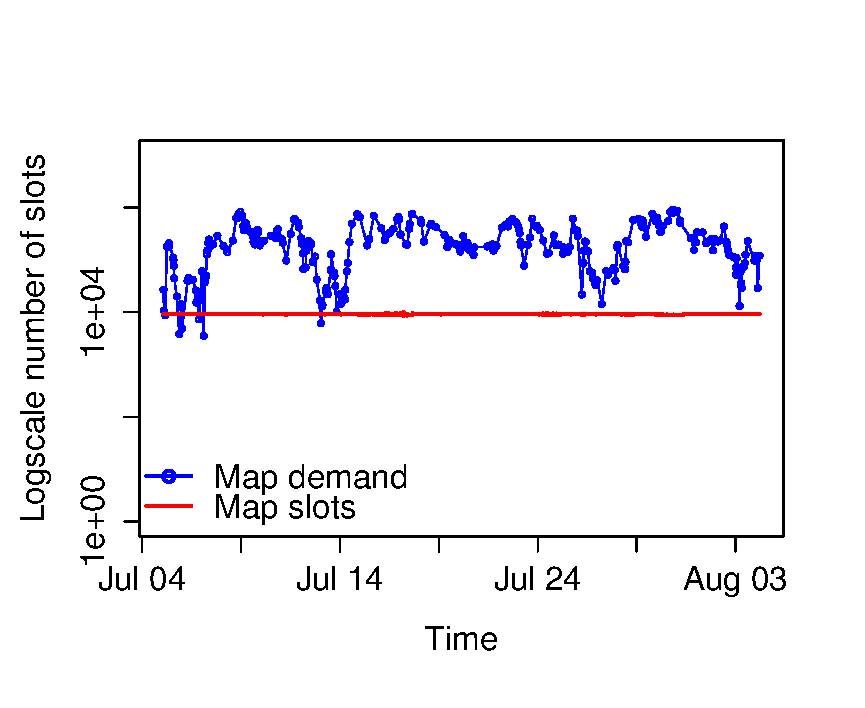
\includegraphics[width=.3\textwidth]{map_demand_and_slots.eps}
        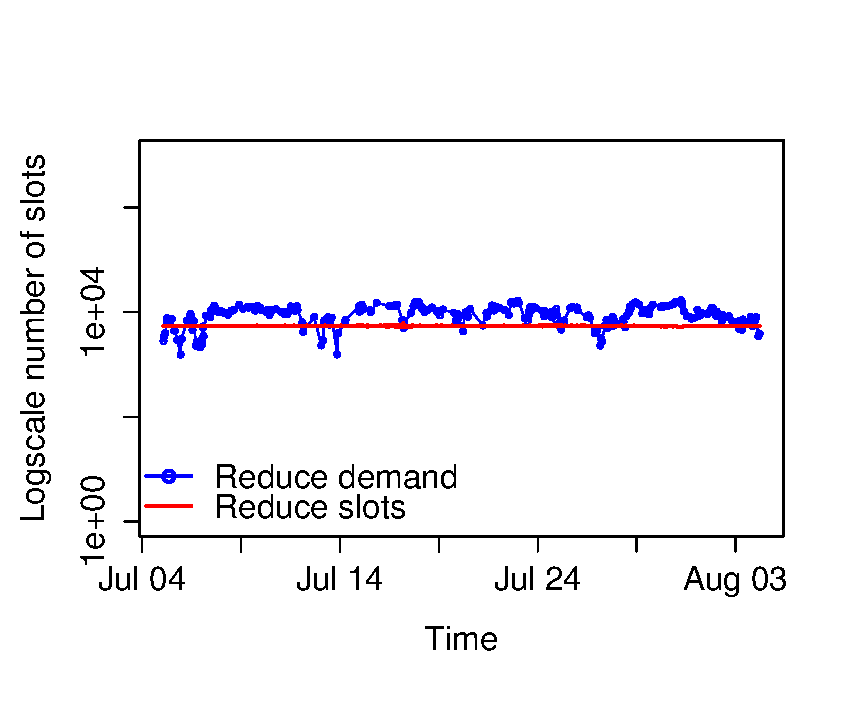
\includegraphics[width=.3\textwidth]{reduce_demand_and_slots.eps}
        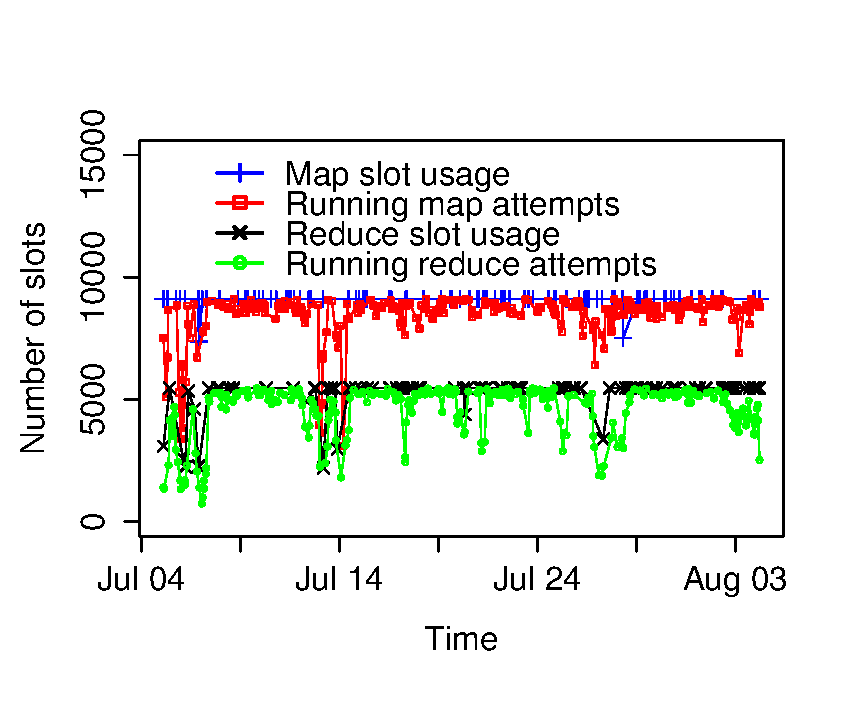
\includegraphics[width=.3\textwidth]{demand_and_running.eps}
        \vspace{-4mm}
        \caption{(a) Map demand (log-scale), (b) Reduce demand (log-scale), and (c) 
 Resource usage on the cluster}
        \vspace{-6mm}
        \label{fig:demand}
\end{figure*}

\noindent {\bf Gatekeepers of Multi-tenancy:}
To meet the conflicting requirements amid different kinds of heterogeneity in a multi-tenant big data system, various mechanisms are used to control how resources are allocated to the applications sharing the cluster. A common technique is to map applications to a set of {\em pools}. Policies are then defined to determine: (a) How are resources distributed across different pools? (b) When is an application admitted to use resources assigned to its pool? (c) How are resources distributed across different applications in the same pool?

These policies can have a huge impact on the performance of a multi-tenant cluster. However, defining policies to achieve good performance is extremely challenging because of the conflicting requirements and the complexities of the system and multi-tenancy. Unfortunately, in practice this responsibility often falls largely on the operations team that manages the cluster, with few effective tools to make data-driven decisions. 

In this paper, we use operational experiences from a large multi-tenant cluster at Rocket Fuel to discuss challenges that operators of these clusters face. Rocket Fuel has a fast-growing Hadoop cluster that currently stores approximately 30 petabytes of data across more than 1000 nodes. Almost all the above types of heterogeneity are seen in this cluster. We break down the challenges in the form of questions that these operators have to answer routinely.  For example:

\squishlist

\item {\em What is the effective utilization of my cluster?} 
We will show in Section \ref{sec:sec2} that the effective utilization of a multi-tenant cluster can be much less than what cluster operators would think based on typical monitoring tools for resource usage.  

\item {\em Should preemption be turned on?} 
The ability for an application X to pre-empt another application Y and start using the resources allocated to Y is one of the configurable policies in multi-tenancy; however, if not used wisely, preemption could lead to significant wasted time and resources.

\item {\em What will be the overall impact of a 10\% increase
in the workload of Pool A?}  
We will show in Section \ref{sec:sec2} that a small increase in the workload of a pool can have a major impact on the performance of applications in another pool in a multi-tenant cluster.

\item {\em What will be the overall impact of changing the data layout
of a table T?}  The application that populates $T$ may belong to a different pool from applications that read from $T$; which in turn could be used to build more tables used by other applications from any pool. These dependencies make the problem of tuning data layouts in a multi-tenant cluster highly challenging.

\squishend

\noindent {\bf Contributions and Roadmap:} 
The above examples come from a large space of questions that human operators have to answer in order to manage multi-tenant clusters effectively. To the best of our knowledge, no single solution exists today that allows operators to ask these questions and get data-driven answers automatically. This paper presents {\em Colossal}, a solution that we have created for this 
problem.

We use real-life examples in Section \ref{sec:sec2} to motivate the challenges that operators of multi-tenant clusters face. Section \ref{sec:sec3} presents Colossal. Section \ref{sec:sec4} discusses related work
and concludes the paper.




\section{Operational Challenges in Multi-tenant Clusters for Big Data
  Analytics}
\label{sec:sec2}

Managed by a small cluster operations team, Rocket Fuel's multi-tenant Hadoop cluster has approximately 1000 nodes storing over 30 petabytes of data. 
The cluster
supports applications created by many teams within the company.
The operations team has created six pools to manage
multi-tenancy. We will call these pools ETL1, ETL2, APP1, APP2, 
BI, and Default. 

\squishlist
\item The ETL1 pool runs a very large number of jobs every day---many of
which are low-level MapReduce jobs---that perform 
data copying and extract-transform-load (ETL) operations.
\item The ETL2 pool contains a mixed workload that includes advanced SQL
analytics, machine-learning computations, ad-hoc queries, and 
repeated workflows. 
\item The APP pools contain ad-hoc or repeated applications
from different teams. 
\item The BI pool contains ad-hoc queries in SQL with considerable 
use of user-defined functions. 
\item The Default pool is for applications that are not mapped
to one of the other pools. 
\squishend

\vspace{1mm}
\noindent Assignment of applications to these pools 
is done statically. Resources are partitioned dynamically 
among the pools based on the fair share resource allocation 
policy as implemented by Hadoop's {\em Fair} 
scheduler \cite{fair-share-scheduler}. 
 As we will discuss later, how resources are partitioned across pools 
and within a pool are based on configurations defined statically 
by the operations team.

Broadly speaking, the objective of the cluster operations team 
is to maximize cluster performance while meeting the business 
service-level agreements (SLAs). 
However, as part of the overall multi-tenant resource management process, 
the cluster operations team has to serve several, potentially
conflicting, interests. For example, users such as business 
analysts (who use the BI pool) wish to minimize the
latency of their jobs; and show little interest in the overall
performance of the cluster. The manager of a team that is 
responsible for a repeated workflow (e.g., one that 
refreshes a base table used by many time-sensitive analysis tasks)
will only care about ensuring that this workflow gets 
enough resources to finish in time. This workflow may be part
of a number of applications that share the ETL2 pool. 

Multi-tenant scenarios like what we see at Rocket Fuel are now 
common in companies that process large amounts of data. 
The larger heterogeneity (recall Section \ref{sec:intro})
and the more democratic nature of Hadoop usage bring 
unprecedented operational challenges compared to managing 
multi-tenancy in traditional parallel database systems.
In the rest of this section, we aim to create a deeper understanding of 
the problems in multi-tenant resource management. We will use real examples 
of problems seen at Rocket Fuel. In particular, we will look at 
these problems from the perspective of Alice. Alice  is 
a fictional member of the cluster operations team who is
responsible for managing multi-tenancy in the cluster. 

\subsection {Understanding Effective Cluster Utilization}
\label{sec:effective-utilization}

Figures \ref{fig:demand}(a) and \ref{fig:demand}(b)
show graphs that Alice looks at routinely
in order to understand the overall demand for resources 
on the cluster. In Hadoop, the resources in the 
cluster are discretized linearly into {\em slots}. The cluster
contains a total {\em MAP\_SLOTS} number of {\em map slots} and 
{\em REDUCE\_SLOTS}  number of {\em reduce slots}. A map (reduce) 
slot can run one map (reduce) attempt at any point of time.

Figure \ref{fig:demand}(a) (Figure \ref{fig:demand}(b))
plots the {\em demand} for map (reduce) slots
in comparison to the total number of map (reduce) slots available. 
This data is for the time from July 5 to August 4, 2014. 
The map (reduce) demand at a time $t$ is defined as the number of map 
(reduce) attempts that are running or ready to run
at time $t$; also called the number of {\em runnable} map (reduce) 
attempts. A runnable map (reduce) attempt will actually run only when it is 
assigned a map (reduce) slot. The number of runnable attempts 
for a logical map or reduce {\em task} can be greater than one if 
{\em speculative execution} is enabled. In this case, Hadoop will 
identify {\em straggler} attempts for a task that are running more
slowly compared to 
other attempts from the same job; and create additional attempts 
that can be run to complete the task.

Alice can see from Figures \ref{fig:demand}(a) and 
\ref{fig:demand}(b) that, at most points of time, the demand 
for slots far exceeds the total number of available slots. 
This observation means that the multi-tenant cluster is 
almost always under contention, so proper management
of resources is essential. The first question that Alice 
usually has is whether the slots available in the cluster are 
all being used as much as possible. 

Figure \ref{fig:demand}(c) plots the actual {\em usage} of
map (reduce) slots for the same time period from July 5 to August 
4, 2014. Map slot usage $U_m(t)$ is defined  at a time $t$ as follows:
\[
U_{m}(t)=\min\left\{S_{m}(t)-C_{m}(t),\mbox{\em MAP\_SLOTS}\right\}
\]
Here, $S_m(t)$ and $C_m(t)$ denote the number of runnable 
map attemts and completed map attempts, respectively, at
time t. Similarly, $U_r(t)$, $S_r(t)$, and $C_r(t)$ are defined for reduce
attempts.

Alice can see from Figure \ref{fig:demand}(c) that the cluster is almost
fully utilized at all points of time. Most cluster operators
would take Figure \ref{fig:demand}(c) to mean that the cluster
is performing fine. However, we will dig deeper to get a sense
of how much useful work is getting done. 
Let us consider the {\em effective cluster utilization}, which 
computes the fraction of cluster usage 
that went into running attempts that were successful and the 
job that they were part of was also successful. 

We can define the effective utilization $E(t)$ of the cluster as the ratio:
\[
E_{m}(t)=\frac{R_{m}(t)}{U_{m}(t)}
\]
where $R_m(t)$ is the number of running map attempts at time $t$
that eventually finished successfully and were also part of a job that 
eventually finished successfully. $E_r(t)$ is defined similarly. 

\begin{figure}
  \centering
  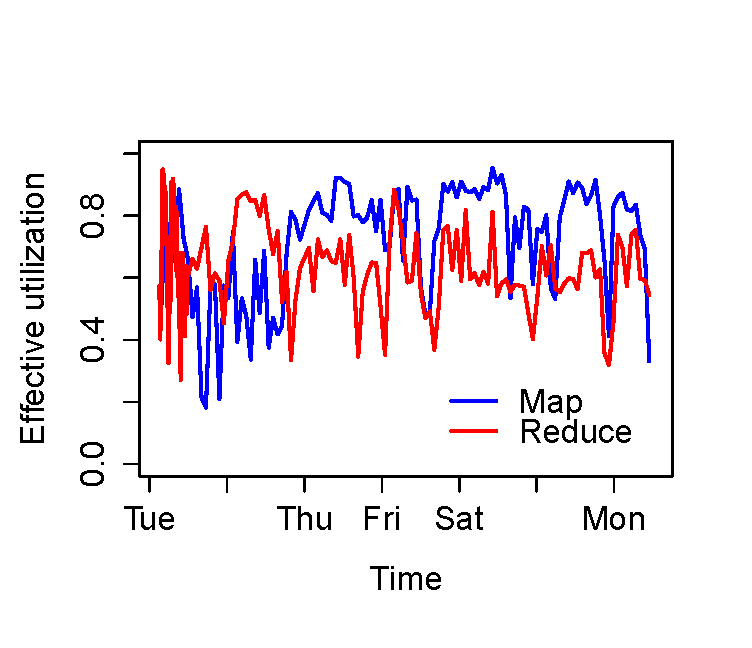
\epsfig{file=eff_util.eps, scale=0.5}
  \caption{Effective map and reduce utilization}
  \label{fig:utilization}
\end{figure}

Figure \ref{fig:utilization} shows $E_m(t)$
and $E_r(t)$ over the week from July 29 to August 4. Alice 
would be surprised by the results in Figure \ref{fig:utilization}:
the average effective utilization for map and reduce is only 72.5\% and
67.3\%, respectively, over this period. Thus, while the cluster 
demand and usage look very high, approximately 30\% of the cluster
resources are being wasted from Alice's perspective. She will 
want to investigate the reasons that are responsible for the 
unexpectedly low effective utilization.
As part of a diagnosis exercise, Alice can generate 
statistics as shown in Table \ref{tab:task-statistics} for 
all the MapReduce jobs run over a one-week period. 

\begin{table}
  \centering
  \caption{Statistics of job and attempt status for a one-week period}
  \begin{tabular}{|c|c|l|} \hline
    Type & Percentage (\%)\\ \hline
    Failed jobs & 3\\ \hline
    Killed jobs & 3.11\\ \hline
    Succeeded jobs & 93.89\\ \hline
    Failed attempts & 0.32\\ \hline
    Killed attempts & 18\\ \hline
    Successful attempts & 81.68\\
    \hline\end{tabular}
    \label{tab:task-statistics}
\end{table}

The table shows that 18.32\% of the 
map and reduce attempts were unsuccessful overall. 
Several factors can lead to unsuccessful attempts. First, 
an attempt will be killed if it is a speculative attempt and the
original attempt for the task has succeeded; or vice versa. Second, 
a MapReduce job can fail due to any number of reasons. Common 
factors include some exception in user code such as a required
file not being found. 

Third, a MapReduce job can be killed by 
the submitting user or by Alice.
A common case seen in practice
is where the job processes heavily-skewed data. Thus, one task
of the job gets hit with a massive amount of data that takes
a very long time to process. Attempts for this task end up causing 
heavy load on the machine where they run, prompting Alice 
to kill the job. A fourth factor is where an attempt gets {\em preempted},
which we will discuss in Section \ref{sec:preemption}. 

\begin{figure}
  \centering
  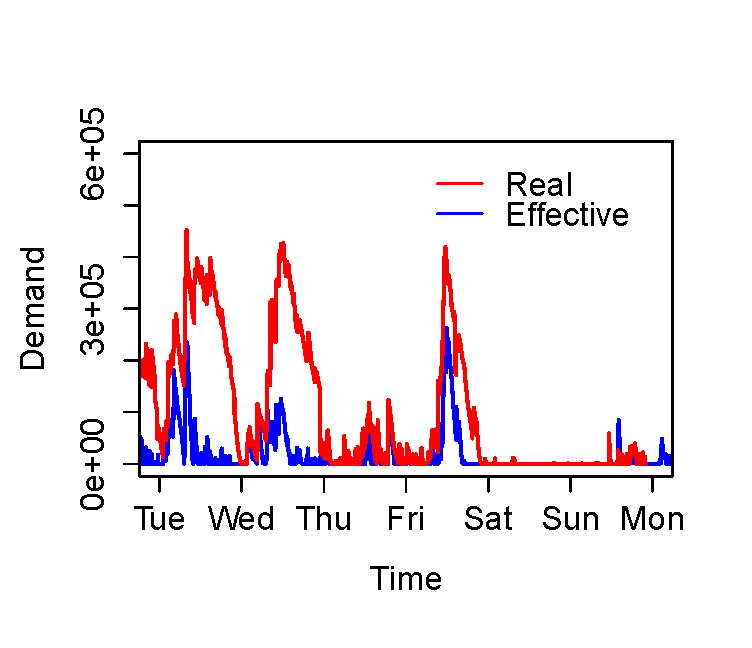
\epsfig{file=analyst_demand.eps,scale=0.5}
  \caption{Map demand of the BI pool}
  \label{fig:BI-demand}
\end{figure}

Figure \ref{fig:BI-demand} shows the map demand in the BI 
pool during the July 29 to August 4 time frame. The ``Real''
plot shows the contributions of this pool 
to the actual map demand, while the ``Effective'' plot
shows the contributions to the effective utilization.
Notice the large gap between the ``Real'' and ``Effective'' plots.
Thus, from Figure \ref{fig:BI-demand}, Alice can conclude that 
the BI pool was one of the contributors to the low effective
utilization seen in the cluster. Applications in the BI pool 
tend to be ad-hoc queries over very large datasets, and 
submitted by users who are not expert users of Hadoop or SQL. 

\eat{
\begin{figure}
  \centering \epsfig{file=CIDR1.eps,scale=0.23}
  \caption{Interactions across pools}
  \label{fig:analyst-Vs-modeling}
\end{figure}
}

\begin{figure}[t!]
        \centering
        \includegraphics[width=.45\textwidth,height=4.5in]{CIDR2.eps}
        \vspace{-4mm}
        \caption{Interactions across pools}
        \label{fig:analyst-Vs-modeling}
        \vspace{-6mm}
\end{figure}

\subsection {Interactions Across Pools}
Different applications in a pool contend for the same set of resources. 
However, can applications in one pool affect those in another pool?
Figure \ref{fig:analyst-Vs-modeling} shows four performance metrics 
for the pools at Rocket Fuel for a week-long interval. In each
case, the blue, purple, and green areas represents the BI, ETL2, 
and APP2 pools respectively. The following observations can be made 
from Figure \ref{fig:analyst-Vs-modeling} as we go through 
the four performance metrics from top to bottom: 

\squishlist

\item During July 6 and 7, the BI and APP2 pools had a slight increase 
in ``Jobs Submitted'', which is the number of jobs being submitted.
\item During the same dates, the BI pool had a more noticeable 
increase in ``Total Cluster Time'', which is the amount of time 
that applications in each pool spend on the cluster. 
\item The last two performance metrics shown---namely, ``Slot Kill Time"
and ``Slot Fail Time''---denote the amount of time consumed by 
attempts that are eventually unsuccessful. Note how these numbers
went up for the BI and APP2 pools. But much more noticeable is how these
times went up for the ETL2 pool. 

\squishend 

Figure \ref{fig:analyst-Vs-modeling} illustrates the importance of 
answering one common type of question that Alice has to answer:
{\em What will be the impact of an $\alpha$\% increase in the workload in 
the Pool $X$?} This question evolves into a number of other 
questions because the workload can increase in different ways. 
For example, natural growth of data sizes can lead to more attempts
or to more running time per attempt. Or, creation of a new BI application
can lead to an increase in the number of jobs being submitted to 
the BI pool. Avoiding these questions or providing cursory 
answers can have catastrophic consequences on cluster performance. 


\begin{table}
  \centering
  \caption{Configuration parameters for BI pool}
  \begin{tabular}{|c|c|l|} \hline
    Name & Setting \\ \hline
  min\_share\_timeout & 2 hours\\ \hline
                  fair\_share\_timeout & 15 minutes\\ \hline
                  weight & 2.0 \\ \hline
                  map\_min\_share & 2287 slots \\ \hline
                  reduce\_min\_share & 1372 slots \\ \hline
                  sched\_mode & FAIR \\ \hline
    \hline\end{tabular}
    \label{tab:scheduler-config}
\end{table}

\subsection{Controlling the Resource Allocation}
\label{sec:preemption}

Table \ref{tab:scheduler-config} shows the configuration 
parameters per pool that control how Hadoop's Fair
scheduler allocates resources across different pools. 
The ``min share'' and ``weight'' parameters control how the
policy of fair sharing is applied by the 
Fair scheduler. Choosing the settings 
for these parameters that provide the best overall 
workload performance is a challenging task that Alice faces. 
The task becomes even more challenging while 
forecasting growth in the demand for different pools, 
and planning for the resources in advance.

Because of space constraints, we will give only one example, namely, 
regarding the impact of preemptions done by the Fair scheduler.
Premption occurs when the number of slots allocated to a pool goes 
below its {\em minimum share} or half its {\em fair share}
for a certain time interval. During preemption, the 
Fair scheduler will kill the most recently launched attempts in pools 
that have more attempts running than their fair shares. The work 
done by the prempted attempts will be lost when they are killed.

The per-pool ``timeout'' parameters shown in Table \ref{tab:scheduler-config}
determine the time interval mentioned above for which a 
pool will wait before preemptions start. 
Alice usually finds it hard to determine whether to enable preemption and, 
if so, what timeout values to set. On one hand, turning on
preemptions is beneficial for performance-critical pools
to meet SLAs. However, preemption leads to wasted work. 
The best setting depends on SLAs, the workload, and cluster capacity. 

To illustrate the challenges here, Figure \ref{fig:preemption} shows the 
reduce fair share and number of 
running reduce attempts in the ETL2 pool over one day. As can be seen,
the ETL2 pool uses more reduce slots than its reduce fair share over
a five-hour interval. This trend will be surprising to Alice
because preemption of attempts is indeed enabled at Rocket Fuel. 
The reason for the trend seen in Figure \ref{fig:preemption} 
is a combination of the fact that the ETL2 pool has very long-running
reduce tasks and the fact that attempts are preempted
in increasing order of their running time so far. Given 
the characteristics of the workload seen in this pool, 
not enabling preemption could impact severely the chances of 
meeting SLAs in other pools. 

\begin{figure}
  \centering
  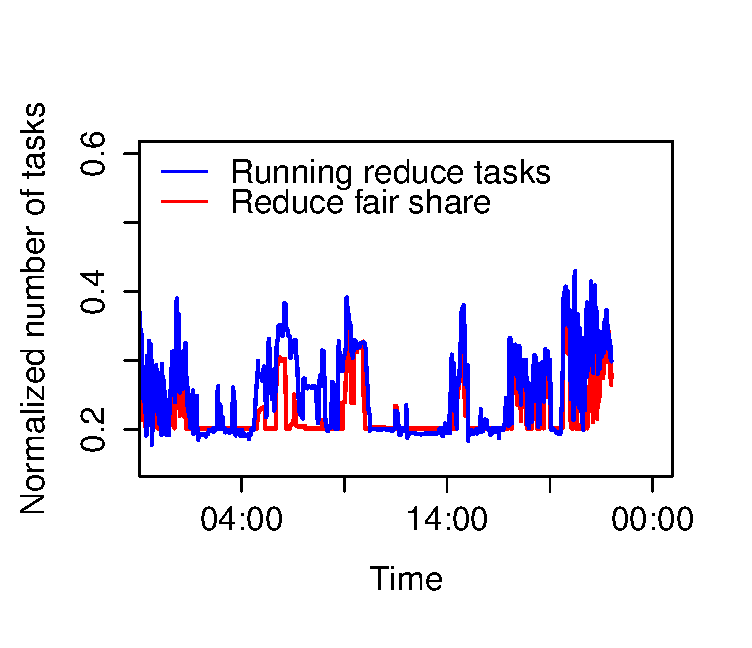
\epsfig{file=long_running_reduces.eps,scale=0.5}
  \caption{Consequences of long-running reduce attempts 
           in the ETL2 pool}
  \label{fig:preemption}
  \vspace{-5mm}
\end{figure}

\subsection{Tuning the Workload in One or More Pools}

Adjusting the per-pool configurations like the ones
in Table \ref{tab:scheduler-config} and Section \ref{sec:preemption}
will enable Alice to control the multi-tenancy. However, 
she would still be playing a {\em zero-sum game} 
because giving more resources to one pool means 
taking away resources from another pool in a contended 
cluster. In this section, we point out five 
different ways in which Alice can make it a 
non-zero-sum game by changing the workload in one or more pools.

\vspace{1mm}
\noindent {\bf Application tuning:}
Tuning queries or jobs in a pool can improve the 
resource usage within the pool as well as free up resources 
for other pools. 

\vspace{1mm}
\noindent {\bf Data layout tuning:}
Tuning data layouts---e.g., changing a table from a text-based 
format to an encoded columnar format---can change the workload
that hits multiple pools. It can be very hard for Alice
to predict the impact of such tuning on the overall multi-tenant
cluster. 

\vspace{1mm}
\noindent {\bf Dependency awareness:}
Analytics workloads can have a number of data-related
dependencies. For example, the input of one job may come 
from another job in a workflow that contains both jobs.
Such dependencies can have significant impact on 
effective utilization. Consider a MapReduce job that 
has long-running map attempts. If reduce attempts for this 
job are started before all map attempts finish, then 
these reduce attempts may not do any useful work for long periods; 
while holding on to slots all the while. We have seen significant 
benefits at Rocket Fuel through tuning that accounts for this behavior. 

\vspace{1mm}
\noindent {\bf Workload shifting:}
As we can see from Figures 
\ref{fig:demand}(a) and \ref{fig:demand}(b), the resource
demand on the cluster has highs and lows. Some of the workloads---e.g., 
those coming from batch applications such as report generation---can
be moved to intervals with low resource demand. 

\vspace{1mm}
\noindent {\bf Admission control:}
Admission control can limit the concurrency level of a pool. 
However, it can be nontrivial for Alice to come up with good
admission control policies given different workload characteristics
per pool as well interactions among pools. We have experienced cases 
where changing the admission control policies for one pool 
led to significant changes in the performance of another pool. 









\section{Our Colossal Approach}
\label{sec:sec3}

As we illustrated in Section \ref{sec:sec2}, the cluster operations
team has to answer a large number of questions in order to manage
multi-tenancy. Broadly, we can categorize these questions into
three categories. 

\squishlist

\item {\em What-is questions:} These are questions aimed at gaining
a deeper understanding of multi-tenancy in the cluster. Examples 
that we saw in Section \ref{sec:sec2} include 
understanding the effective utilization of the overall cluster 
as well as the effective utilization of different pools. 

\item {\em What-if questions:} These are questions aimed 
at understanding the impact of various changes. Examples include
understanding the impact of: (a) an increase in a pool's 
workload, (b) a change in a pool-level configuration
parameter such as the preemption timeout, 
and (c) a change in the layout of a table.

\item {\em What-should questions:}  These are questions aimed 
at identifying the best configurations for tunable parameters
given constraints and/or an optimization objective. 
An example is to find the best setting of pool-level 
configuration parameters for all pools in order to satisfy 
constraints (SLAs) on average completion time in some pools, 
while maximizing the overall cluster utilization. 

\squishend

{\em Colossal} is a platform that we are developing to 
enable cluster operators to get answers to such questions 
easily. In this section, we will describe the five main
components of Colossal and our current implementation of each component. 
Each component is designed to be pluggable and can have different 
implementations.

\subsection{Extractors}
An {\em Extractor}'s goal is to generate a workload model
from raw traces of workload execution. The main reason
for generating workload models is to enable anwering
What-if questions of the form: what is the impact of  
a 5\% increase in the workload of the BI pool? 
Workload models enable concrete descriptions of 
what a 5\% increase in a particular workload means.  

We have implemented an Extractor for the workload 
seen on Rocket Fuel's multi-tenant cluster. This Extractor
takes as input all job history logs generated
by Hadoop for some period of time. From a statistical analysis
of the workload, we observed that the job
arrival follows a Poisson process with a relatively constant
arrival rate for each pool. In addition, the map and reduce attempt
duration follows a lognormal distribution (which is similar
to the observations in \cite{taobao-paper}). 
The task count of a job can also be approximated using a lognormal
distribution for each pool. Thus, the Extractor uses 
maximum likelihood estimation of parameters to fit 
the observed distributions. Table \ref{tab:workload-model}
shows the best-fit workload model for the BI pool.

\begin{table*}
  \centering
  \caption{Workload model of analyst pool (Time is in seconds)}
  \begin{tabular}{|c|c|l|} \hline
    Parameter&Description&Estimated Value\\ \hline
    job\_arrival\_rate & Number of job arrivals per second &
    0.00282392166\\ \hline
    logmean\_maps\_per\_job & Mean of the logarithm of job map count & 4.860108\\ \hline
    logmean\_reduces\_per\_job & Mean of the logarithm of job reduce count & 1.720507\\ \hline
    logsd\_maps\_per\_job & Standard deviation of the logarithm of job map count & 3.202215\\ \hline
    logsd\_reduces\_per\_job & Standard deviation of the logarithm of job reduce count & 2.540193\\ \hline
    logmean\_map\_duration & Mean of the logarithm of job task duration & 3.765196\\ \hline
    logmean\_reduce\_duration & Mean of the logarithm of reduce task duration & 5.154496\\ \hline
    logsd\_map\_duration & Standard deviation of the logarithm of map task duration & 0.8837955\\ \hline
    logsd\_reduce\_duration & Standard deviation of the logarithm of reduce task duration & 2.043326\\ \hline
\end{tabular}
\label{tab:workload-model}
\end{table*}

\subsection{Transformers}
A {\em Transformer}'s goal is to generate an actual 
specification of a workload that will be input  
to the {\em Predictor}. We have implemented two different
Transformers so far. A simple Transformer takes the 
raw Hadoop job history logs and transforms it to the 
workload input specification supported by the Predictor. 
The more complex Transformer that we have implemented 
can take the workload model learned by the Extractor 
from the previous section, and generate various scaled versions
of the workload along different dimensions. For example, 
this Transformer can generate a workload 
with a 5\% increase in the number of map tasks per job
in order to represent a 5\% increase in overall
data volume. 

In future, we will be supporting more sophisticated
Transformers to connect Colossal with other tuning tools
in order to answer questions of the form: What will be the overall 
impact of changing the data layout of a table $T$? 
To answer this question, a data-layout tuning tool (external
to Colossal) will have to provide Colossal's Predictor with 
the new workload that will result from 
changing the data layout of table $T$. In this way, Colossal
will be able to apply a divide-and-conquer approach to 
answer hard questions in multi-tenancy that cluster operators 
have no way of answering today. 

\subsection{Predictors}
A {\em Predictor} takes three inputs: (i) a multi-tenant workload, 
(ii) pools and their configuration, and (iii) 
cluster resource configuration. The goal of the Predictor
is to output the predicted schedule of execution
of the workload on the cluster. In addition, the Predictor
also outputs standard performance metrics associated with 
a multi-tenant workload. 

The Predictor has to be both fairly accurate as well as 
highly efficient in performance prediction. As we will 
see in Section \ref{sec:optimizer}, {\em Optimizers} may have 
to call the Predictor multiple times. We could not 
use a number of Hadoop simulators that have 
been developed in the past either because they 
were inefficient in handling large workloads or 
were too inaccurate due to assumptions made 
regarding multi-tenancy \cite{sls,mr-sim}. 

Our current implementation of the Predictor is for a 
cluster where the multi-tenancy is enforced by the Hadoop
Fair scheduler. This Predictor is based on a novel algorithm
which simulates the Fair scheduler in accelerated {\em virtual
time}. Given the workload trace for an interval $T$, the predictive
algorithm will require a much shorter run-time $t$ << $T$ to produce the
predicted results. For example, the Predictor requires less than 
4 minutes (a significant fraction of which is I/O time for 
the large workload file) to generate 
performance predictions for one week of Rocket Fuel's workload.

The key idea used in the predictive algorithm is to map events---such as
preemptions, job starts, and job completions---on to a virtual timeline. A
finite state machine is then established to process the events in the
increasing order of virtual time. While processing an event, the state
machine may also alter later events in the virtual timeline, but
not the earlier ones. Thus, the running time of the algorithm is
proportional to the number of tasks, jobs, and preemptions.
This approach has
the advantage over most previous approaches in which the running time of
simulation also depends on the running time of jobs
\cite{sls,conf/cluster/VermaCC11,mr-sim}.

\subsection{Inspectors}

Once the Predictor or Optimizer 
has generated its output, an {\em Inspector}'s
role is to help the operations team get the answer to 
their question from the output. In many cases, the 
overall understanding of the operations team can be further improved by 
visualizing the time series of metrics in the output. 
Our current implementation of Inspectors 
provides visualizations for several built-in performance metrics 
such as effective utilization as
described in the previous section, average job latency for
each pool, and others. 

\begin{figure}
  \centering 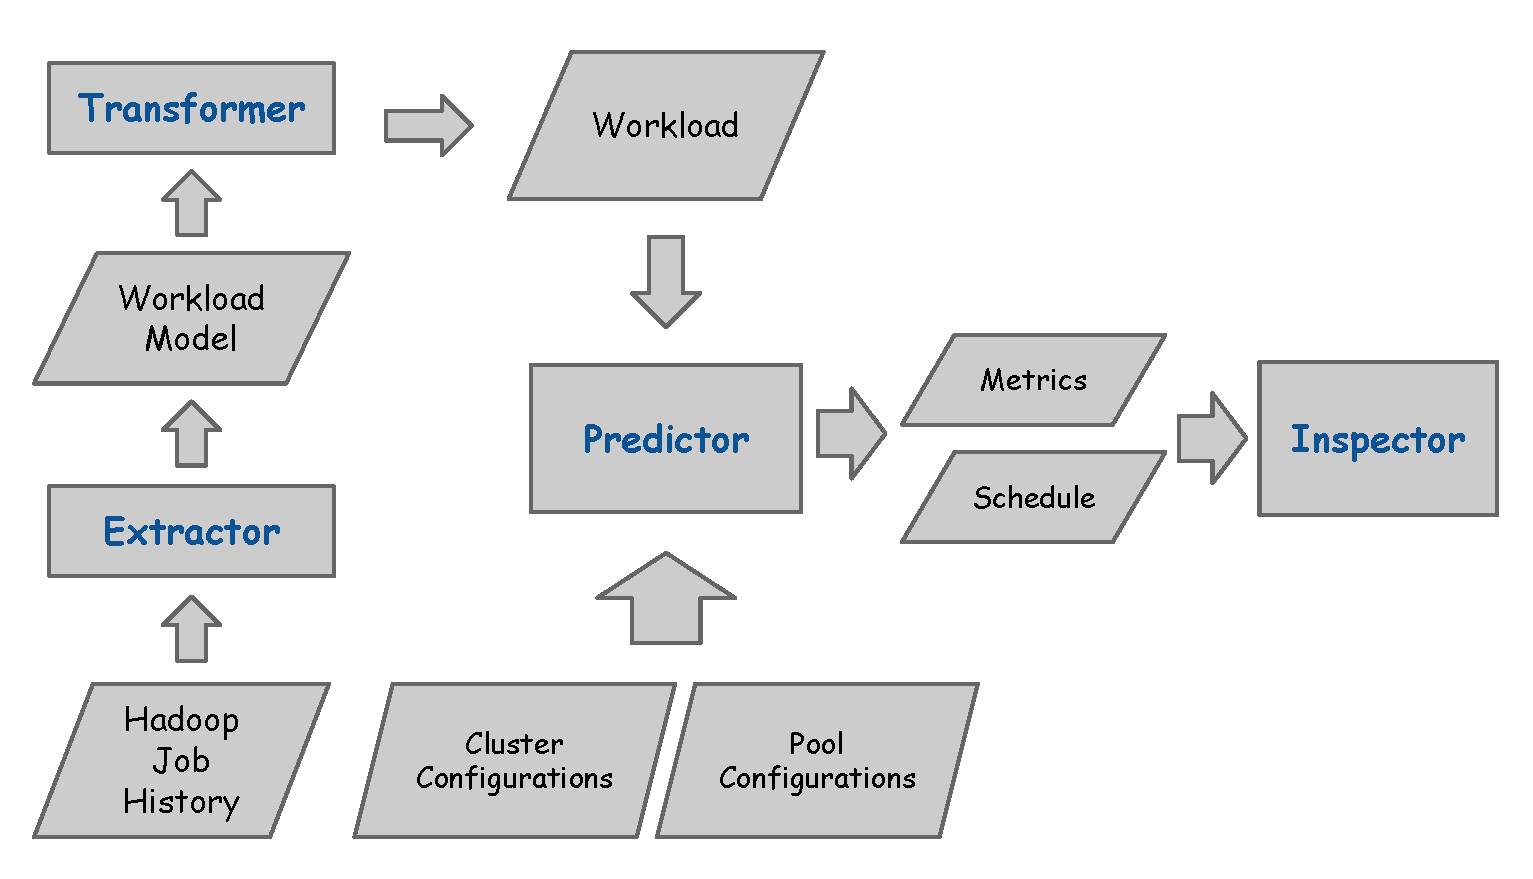
\epsfig{file=arch.eps,scale=0.3}
  \caption{Overview of the Colossal Platform}
  \vspace{-6mm}
\end{figure}

\subsection{Optimizers}
\label{sec:optimizer}

The role of an {\em Optimizer} in the 
Colossal platform is to find configuration parameter settings that 
optimize user-specified performance metrics
in a multi-tenant cluster. The optimization is done by 
searching over the possible parameter space, and 
calling into the Predictor in order to estimate performance
for selected configuration parameter settings. The search process 
is made efficient by parallelizing using MapReduce as well as 
using heuristics to prune the search space dynamically.

Specifically, a user can define an objective function {\em F(M,S)} 
where $M$ and $S$ are, respectively, the output metrics and
schedule from the Predictor. Typical objective functions use
three of the built-in metrics:
(a) {\em AvgJobLatency}, which represents the average job
latency of each pool, (b) {\em Throughput}, which represents the throughput
(number of jobs per second) of each pool, and (c) {\em EffectiveUtil}, 
which represents the effective utilization defined in 
Section \ref{sec:sec2}. Additionally,  users 
specify the parameters (i.e., the free variables in the search) 
for which they want recommended settings. For example, 
any subset of the configuration parameters listed in 
Table \ref{tab:scheduler-config} can be specified 
as free variables. 




\section{Discussion and Related Work}
\label{sec:sec4}

Efficient processing of big data has given rise to multi-tenant, big data clusters where multiple applications run on and share the same resources and data. Such multi-tenancy poses significant challenges for human operators of the cluster to tune the cluster to meet performance requirements that often conflict each other. The research and open-source communities 
are doing a lot of work in this area. The main threads of 
work include: (a) building cluster operating systems 
like Mesos \cite{mesos} and YARN \cite{yarn}
that have the resource provisioning and 
isolation mechanisms to support multi-tenancy; (b) 
algorithms and policies to allocate resources in ways that are 
efficient as well as fair to all tenants \cite{conf/cidr/NarasayyaDSCC13,ghodsi11,isard09}; and (c) ability to support multiple tenants
on as few software and hardware resources as possible 
(e.g., \cite{DBLP:journals/pvldb/DasNLS13}).

In this paper, we observed that, in practice, the responsibility 
of managing multi-tenancy falls largely on the operations team that 
manages a  multi-tenant cluster. 
We used operational experiences from a large, multi-tenant 
cluster to discuss the challenges that arise. Specifically, 
we observed that cluster operators have 
few effective tools to make data-driven decisions
while managing multi-tenancy. We described 
Colossal, a platform that we have developed to address this gap. 

Space contraints precluded us from presenting results from an experimental
evaluation. Overall, the primary advantages that Colossal 
offers are: 
\begin{itemize}

\item{\em Efficiency}: Colossal can predict, with acceptable 
levels of accuracy, the performance metrics and schedule
of one week's workload at Rocket Fuel 
(approximately, 55,000+ MapReduce jobs and 36 million attempts) in
under four minutes on a commodity machine.

\item{\em Flexibility}: Colossal allows for easy abstraction, modification, 
and prediction of the workload over any specified time period lengths.

\item{\em Modularity}: The components that generate the 
workload as well as predicted performance metrics
are pluggable. Thus, Colossal can be customized based on the 
characteristics and needs of different multi-tenant environments. 

\end{itemize}




%\vspace{-3mm}

{
\small
%\singlespacing
\bibliographystyle{abbrv}
\bibliography{paper}
}
%\vspace{-4mm}
%\appendix

%\clearpage
%\appendix
\section{Demonstration Proposal}

\subsection{Colossal-based solutions}
Overall, Colossal supports 1) simulating the performance of the
cluster under given workload and configuration, 2) modeling the
workload and allowing for modifications, and 3) automatic parameter
tuning based on given performance metrics. Specifically, 1) is
achieved using the pluggable scheduler simulator in Colossal, 2) is
done by fitting a statistical model to historical workload traces,
and 3) relies on 1) to perform exhaustive or heuristic search over
the parameter space.

As a proof-of-concept, we have implemented a prototype of ...

We will first describe the design of the prototype system.
Then, we describe how we will demonstrate the 
prototype system to motivate and illustrate the ...

\vspace{-1mm}
\subsection{Description of Prototype System}


Colossal is designed to answer ``What-If'' questions concerning the
cluster performance, workload, and parameters. The general steps to
pose a ``What-If'' question are shown in Fig 5. First, workload is
either extracted from Hadoop job history or generated using the
workload model. Second, the simulator inputs the workload and
cluster configurations, and then outputs a performance metrics
file, which is similar to Hadoop metrics, as well as the schedule.

\subsubsection{Posing a question in Colossal}
To pose performance related questions, one simply needs to
visualize the metrics time series in the metric file, or
alternatively to analyze the schedule. Colossal provides several
built-in performance metrics, such as effective utilization as
described in the previous section and the average job latency for
each pool. To pose questions concerning the workload, the
statistical workload model introduced in 3.1 is readily available
for modifications. As for automatic parameter tuning, one can fix
the objective, e.g., average job latency of analyst pool, and then
repeat the simulation against different parameter combinations. In
this case, constraints can also be specified by the user in a
similar manner. This is useful to guarantee the SLAs of production
jobs.




Figure~\ref{} shows the architectural overview of the 

Specifically, there are two components that we have developed: 

\vspace{1mm}
\noindent\textbf{TBD:}

\vspace{1mm}
\noindent\textbf{TBD:} 

\vspace{-1mm}
\subsection{Outline of Demonstration Plan}
The demonstration will consist of three parts. First, we will show how to ..

Second, we will also show how 

Finally, we will show the 


\begin{table*}
  \centering
  \caption{Procedures to pose questions in Colossal}
  \begin{tabular}{|p{6cm}|p{10cm}|l|} \hline
    Question&Procedures\\ \hline
    What is the effective utilization of the cluster?& Use the
    simulator to generate the schedule files. Then use built-in
    function EffUtil(S) to obtain the effective utilization based on
    S.\\ \hline
    What is the impact of a change in workload?& Reflect the change in
    the workload model, and then run Colossal to generate metrics and
    schedule files. Next, compute the performance metrics of interest
    based on these two files.\\ \hline
    Should preemptions be turned off?& First, visualize the metrics
    file generated by Colossal for the present workload. Then identify
    any long-running tasks problem in any pools. Next, compare the
    performance before and after turning off the preemptions. Finally,
    make a decision according to above results.\\ \hline
    How to evaluate the impact of a 5\% increase in the workload of
    analyst pool?& First, run Colossal to obtain baseline performance
    using any user-defined metrics. Then increase the job arrival rate
    of analyst pool by 5\% and re-evaluate the performance. Finally,
    compare the results above.\\ \hline
    How loosening the admission control of modeling pool impacts the
    performance?& Another module is needed to map the original
    workload to an adjusted one according to the loosened admission
    control. Then use Colossal to evaluate the performance using the
    adjusted workload.\\ \hline
    What difference does ORC format make? & Likewise, another module
    is needed to produce the adjusted workload and use Colossal to
    evaluate the performance of the adjusted workload.\\ \hline
  \end{tabular}
\end{table*}


The Colossal answers questions as
described in Section 2. These questions are first translated and then
effected on the workload model. The simulator processes the workload
generated by the workload model and outputs the schedule and
performance metrics for evaluation. 

Colossal is designed to answer ``What-If'' questions concerning the
cluster performance, workload, and parameters. The general steps to
pose a ``What-If'' question are shown in Fig 5. First, workload is
either extracted from Hadoop job history or generated using the
workload model. Second, the simulator inputs the workload and
cluster configurations, and then outputs a performance metrics
file, which is similar to Hadoop metrics, as well as the schedule.



As for automatic parameter tuning, one can fix
the objective, e.g., average job latency of analyst pool, and then
repeat the simulation against different parameter combinations. In
this case, constraints can also be specified by the user in a
similar manner. This is useful to guarantee the SLAs of production
jobs.





\end{document}
